\documentclass[a4paper]{article}
\setlength{\parindent}{0pt}

%%%%%%%% CREATE DOCUMENT STRUCTURE %%%%%%%%
%% Language and font encodings
\usepackage[english]{babel}
\usepackage[utf8x]{inputenc}
\usepackage[T1]{fontenc}
%\usepackage{subfig}

%% Sets page size and margins
\usepackage[a4paper,top=3cm,bottom=2cm,left=2cm,right=2cm,marginparwidth=1.75cm]{geometry}

\usepackage{tikz}
\usetikzlibrary{arrows, shapes.geometric, intersections}

\tikzstyle{smallbuilding} = [rectangle, rounded corners, minimum width=4cm, minimum height=1.5cm,text centered, draw=black, fill=red!30]
%\tikzstyle{code} = [trapezium, trapezium left angle=70, trapezium right angle=110 , minimum width=3cm, minimum height=1cm, text centered, draw=black, fill=blue!30]
\tikzstyle{mediumbuilding} = [rectangle, minimum width=3cm, minimum height=1cm, text centered, draw=black, fill=green!30]
\tikzstyle{largebuilding} = [rectangle, minimum width=3cm, minimum height=1cm, text centered, draw=black, fill=orange!30]


%% Useful packages
\usepackage{framed}
\usepackage{amsmath}
\usepackage{graphicx}
%\usepackage[colorinlistoftodos]{todonotes}
\usepackage[colorlinks=true, allcolors=blue]{hyperref}
\usepackage{caption}
\usepackage{subcaption}
\usepackage{listings}
\usepackage{lstautogobble}
\usepackage{sectsty}
\usepackage{apacite}
\usepackage{float}
\usepackage{titling} 
\usepackage{blindtext}
\usepackage[square,sort,comma,numbers]{natbib}
\usepackage{xcolor}
\definecolor{darkgreen}{rgb}{0.0, 0.4, 0.0}

\definecolor{pblue}{rgb}{0.13,0.13,1}
\definecolor{pgreen}{rgb}{0,0.5,0}
\definecolor{pred}{rgb}{0.9,0,0}
\definecolor{pgrey}{rgb}{0.46,0.45,0.48}

\usepackage{listings}
\lstset{language=Java,
    showspaces=false,
    showtabs=false,
    breaklines=true,
    showstringspaces=false,
    breakatwhitespace=true,
    commentstyle=\color{pgreen},
    keywordstyle=\color{pblue},
    stringstyle=\color{pred},
    basicstyle=\ttfamily,
    colframe=white!75!black,
    moredelim=[is][\textcolor{pgrey}]{\%\%}{\%\%}
}

\usepackage[most]{tcolorbox}

\newtcblisting{shell}{colback=black,colupper=white,colframe=white!75!black,
	listing only,listing options={language=sh}}

% ToDo: List
\usepackage{enumitem,amssymb}
\newlist{todolist}{itemize}{2}
\setlist[todolist]{label=$\square$}

%%%%%%%% DOCUMENT %%%%%%%%
\begin{document}

%%%% Title Page
\begin{titlepage}

\newcommand{\HRule}{\rule{\linewidth}{0.5mm}} 							% horizontal line and its thickness
\center 
 
% University
\textsc{\LARGE University of Illinois @ Urbana-Champaign}\\[1cm]

% Document info
\textsc{\Large CI 487: Data Structures for CS Teachers}\\[0.2cm]
\textsc{\large }\\[1cm] 										% Course Code
\HRule \\[0.8cm]
{\huge \bfseries Application 2: Tree Dictionary}\\[0.7cm]								% Assignment
\HRule \\[0.8cm]
\vfill
%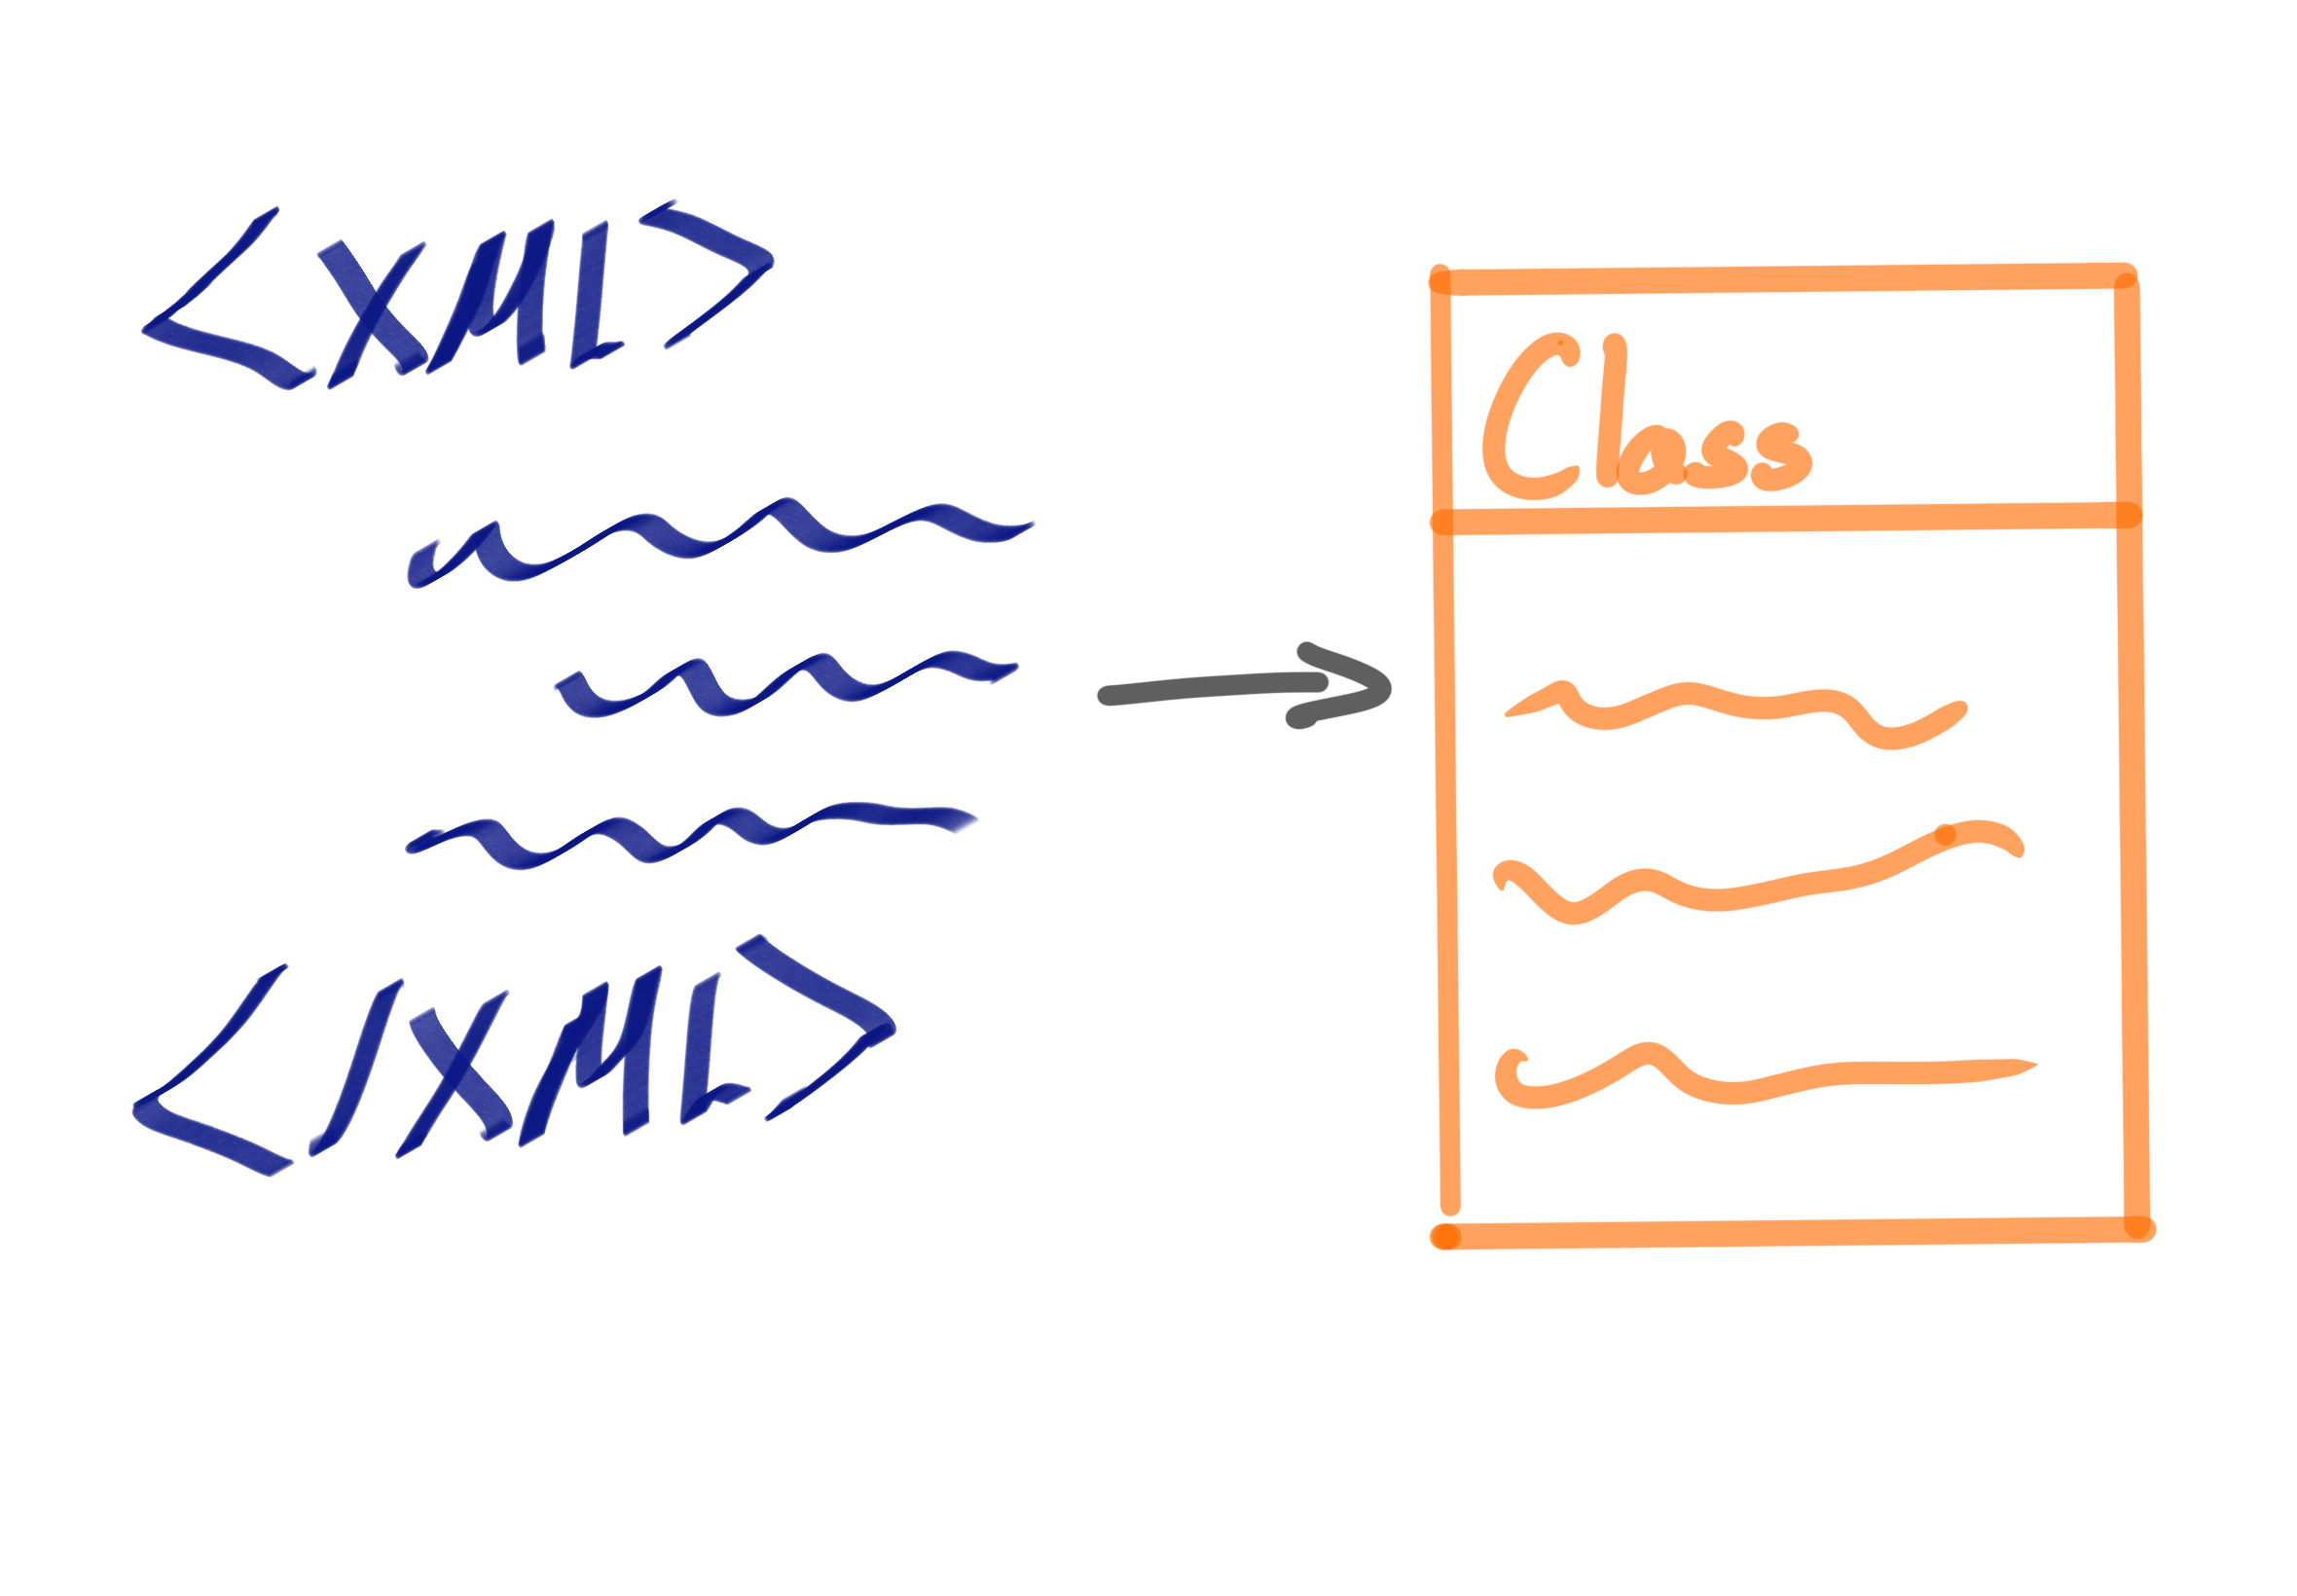
\includegraphics[width=0.6\textwidth]{images/xml.jpg}\\[1cm] 	% University logo
\vfill 
\end{titlepage}


\section*{Objectives and Overview}

Application assignments are intended to be an opportunity to take a step back
use some of the data structures you have been using. It is often easy to get so
bogged down in the details of creating and implementing data structures and not
have the opportunity to use them in performing useful tasks. In this exercise
you will be using an AVL tree similar to the implementation of the one you
implemented last week. You will be using this data structure to implement
a simple dictionary lookup engine. In doing so it has three objectives:

\begin{enumerate}
    \item To introduce you to a situation where storing data in the form of a tree is useful and to use that situation as a method of practicing using trees.
    \item To give you the opportunity to write several classes largely from scratch.
\end{enumerate}

With respect to the last point, the starter files you will be presented for
this assignment are \textit{much} more spare than those you have been given
for past assignments. The code needed to implement these methods will require
far less code than previous assignments and will primarily focus on translating 
the more abstract problem definition into a working program. As such, you are granted
a great deal of freedom in how you complete this assignment and it's core functionality.

\section{Structures and Specifications}

The structure of this assignment will be spread over five separate file:
\begin{enumerate}
    \item AVL.java - The provided AVL tree that you will use to implement your dictionary. This class should be read through but remain unmodified.
    \item DictEntry.java - This will be fundamental unit in our dictionary. Each of these classes will contain some attributes for holding words and definitions, a compare to method for comparing instances of DictEntry, and a toString methods for printing them.
    \item Dictionary.java - This class will hold the AVL tree of DictEntry objects. It will contain a constructor that populates the dictionary with an initial set of works from a file in addition to two methods that allow for searching and insertion into the tree.
    \item Main.java - This will be the class that contains the main method where you will implement the user interactivity with the dictionary.
    \item dict.csv - This is the file of initial comma separated files containing an initial set of words and definitions. Your Main class will use this to create a Dictionary with an initial set of words.
\end{enumerate}

\subsection{Step 0: Reading through AVL.java}

This file contains a correct implementation of the AVL class. You are
encouraged to read through the code in the file prior to proceeding.
Specifically, the following methods:
\begin{enumerate}
    \item \lstinline|public void insert(T data)|: This method inserts some data of generic type into the AVL tree.
    \item \lstinline|public TreeNode<T> search(T data)|: This method finds and returns a node containing some data of generic type T.
\end{enumerate}
Each of these methods will be useful when you implement the
\lstinline|Dictionary|.

\subsection{Step 1: Implementing DictEntry}

The first thing we will need for our dictionary tree is a class that stores a
word and it's definitions. This is what the \lstinline|DictEntry| class will be 
used for. Use the following specifications to implement the class such that it 
contains the attributes and methods we will require in future portions of the 
assignment.

\subsubsection*{Attributes}
The class should have two \lstinline|String| attributes: 1) \lstinline|word|
and 2) \lstinline|definition| each of these attributes should be
\lstinline|private final| as we don't want the user of this class to have
unmoderated access to the attributes and we don't want them being changed after
they are initially set. 

\subsubsection*{Methods}

The following methods should be implemented for this class:
\begin{enumerate}
    \item Create a constructor for \lstinline|DictEntry| that is used to set the \lstinline|word| and \lstinline|definition| attributes when a new instance of the class is created.
    \item Create a getter for each of the attributes
    \item \lstinline|compareTo|: This methods should override the compareTo method in order to allow for two \lstinline|DictEntry| classes to be compared.
    \item \lstinline|toString|: This method should return a string containing the word and it's definition.
\end{enumerate}

You will be implementing these methods from scratch in this assignment so be
sure to look back on your previous assignments for examples.

\subsection{Step 2: Implementing Dictionary}

This class has two core components:
\begin{itemize}
    \item It should have a constructor that takes a String representing a file path as a parameter, read that file, and use its contents to populate the AVL tree.
    \item It should have methods that allow for adding \lstinline|DictEntry|s to the tree and searching the tree.
\end{itemize}
As such, this section will be organized such that the first part will be a walkthrough
on how to read a CSV file with clues on how you can use the data from that file 
to construct the initial dictionary. The second part will be details on the methods you will
implement but, in keeping with the theme of the assignment, you will be implementing these 
methods yourself with reduced skeleton code.

\subsubsection{Implementing the Constructor}

Provided to you is a constructor which takes a single parameter, a string
representing a file path.  That file path should be to a file containing comma
separated values. The structure of the CSV format that this method should
support is a series of lines of the format: \texttt{word,definition}. This 
walkthrough will cover how to: 1) open and iterate over the file and 2) split
each line to extract the word and the definition. 

\paragraph{Creating a File Object: } Reading the file begins with creating a
new instance of a \lstinline|File| object, as shown below.
\begin{lstlisting}[frame=trBL]
File infile = new File(fp);
\end{lstlisting}
As you can see this file object should take 

\paragraph{Using File + Scanner to Read File: } The \lstinline|Scanner| 
class is fundamentally a class that is used to read from  input streams. In the
past, and in this assignment, you primarily use it to read from the
\lstinline|System.in| (i.e., your keyboard). However, you can also provide it 
other input streams, such as the file object you just created, as seen below:
\begin{lstlisting}[frame=trBL]
try{
    fileReader = new Scanner(infile)
} catch (FileNotFoundException e){
    System.out.println("File not found");
    return;
}
\end{lstlisting}
Reading the file with a Scanner can produce a \lstinline|FileNotFoundException|
which Java requires us to catch.

\paragraph{Reading a File: } 

The following loop structure can be used to read the file:
\begin{lstlisting}[frame=trBL]
while(fileReader.hasNextLine()){
    String line = fileReader.nextLine();
    String[] elements = line.split(",");
}
\end{lstlisting}

Each of these methods performs the following:
\begin{itemize}
    \item \lstinline|fileReader.hasNextLine()|: This returns true if the file has a next line and false otherwise.
    \item \lstinline|fileReader.nextLine()|: This gets the next line from the file.
    \item \lstinline|line.split(",")|: This splits a string into an array of strings on the comma (e.g., \lstinline|"word, this is a def."| \ \textrightarrow \ \lstinline|{"word", "this is a def."}|).
\end{itemize}

\textbf{Your Task:} Take the above code segments and integrate them into the
constructor. You will use the result of the line split to create an instance of
\lstinline|DictEntry| each iteration and add it to the dictionary.

\subsubsection*{Methods}

Each of these methods will be very short (1-3 lines) as they will effectively serve as 
wrappers for the AVL tree methods since the \lstinline|dictionary| attribute in the 
class is private.
\begin{enumerate}
    \item \lstinline|lookupWord|: This method should do three things: 1) take a single string word as a parameter, 2) create an instance of \lstinline|DictEntry| with a \lstinline|null| entry for the definition, and 3) use that \lstinline|DictEntry| to call the search method for the AVL tree and return the result. 
    \item \lstinline|addWord|: This method should take two string parameters: A word and a definition. It should then create a new \lstinline|DictEntry| using those parameters and add it to the dictionary.
\end{enumerate}
Each of these methods should have \lstinline|public| access.

\subsection{Step 3: Implementing Main} This will be the main class for
the user to interact with the dictionary. Provided is a line of code that
creates a new instance of a \lstinline|Dictionary| and assigns it to the
variable \lstinline|dict| along with a \lstinline|while(true)| loop in which
you will implement the following interactive structure.
\begin{enumerate}
    \item Ask the user for a word
    \item Use the \lstinline|lookupWord| method from the \lstinline|dict| to lookup that word and store the result
    \item If the results are \lstinline|null| indicating that the word was not found you should...
        \begin{enumerate}
            \item Ask the user if they want to add the word to the dictionary. 
            \item If they do ask them for the definition and use the \lstinline|addWord| method to add that word and associated definition to the dictionary.
        \end{enumerate}
    \item If the results weren't \lstinline|null| (i.e., the word was found) then you should print the word entry.
\end{enumerate}

\end{document}
